%%%%%%%%%%%%%%%%%%%% author.tex %%%%%%%%%%%%%%%%%%%%%%%%%%%%%%%%%%%
%
% sample root file for your "contribution" to a contributed volume
%
% Use this file as a template for your own input.
%
%%%%%%%%%%%%%%%% Springer %%%%%%%%%%%%%%%%%%%%%%%%%%%%%%%%%%%%%%%%%


%% RECOMMENDED %%%%%%%%%%%%%%%%%%%%%%%%%%%%%%%%%%%%%%%%%%%%%%%%%%%
\documentclass[graybox]{svmult}
%
%% choose options for [] as required from the list
%% in the Reference Guide
%
\usepackage{mathptmx}       % selects Times Roman as basic font
\usepackage{helvet}         % selects Helvetica as sans-serif font
\usepackage{courier}        % selects Courier as typewriter font
\usepackage{type1cm}        % activate if the above 3 fonts are
                             % not available on your system

\usepackage{makeidx}         % allows index generation
\usepackage{graphicx}        % standard LaTeX graphics tool
                             % when including figure files
\usepackage{multicol}        % used for the two-column index
\usepackage[bottom]{footmisc}% places footnotes at page bottom

%% see the list of further useful packages
%% in the Reference Guide
%
%\makeindex             % used for the subject index
%                       % please use the style svind.ist with
%                       % your makeindex program
%
%%%%%%%%%%%%%%%%%%%%%%%%%%%%%%%%%%%%%%%%%%%%%%%%%%%%%%%%%%%%%%%%%%%%%%%%%%%%%%%%%%%%%%%%%%
%

\usepackage{amsmath}
\usepackage{booktabs}
\usepackage{algorithm,algpseudocode}

\begin{document}


\title*{Almost Exact Mixed Scheme for Gatheral Double Mean Reverting Model}
% Use \titlerunning{Short Title} for an abbreviated version of
% your contribution title if the original one is too long



 \author{Ayoub Haida, Mara Kalicanin Dimitrov, Tilemachos Marmaras and Ying Ni\orcidID{0000-0002-0835-7536} }

\institute{Ayoub Haida, Mara Kalicanin Dimitrov, Tilemachos Marmaras and Ying Ni \at Division of Mathematics and Physics M\"{a}lardalen University, SE 721 23 V\"{a}ster{\aa}s, Sweden,  \email{ayoub.haida@mdu.se, mara.kalicanin.dimitrov@mdu.se, tilemachos.marmaras@gmail.com, ying.ni@mdu.se}
}

 
% Use \authorrunning{Short Title} for an abbreviated version of
% your contribution title if the original one is too long
%\institute{\at Mälardalens University, Universitetsplan 1, Västerås, Sweden, \email{ayoub.haida@mdu.se}
%\and \at Mälardalens University, Universitetsplan 1, Västerås, Sweden, \email{mara.kalicanin.dimitrov@mdu.se}}

%
% Use the package "url.sty" to avoid
% problems with special characters
% used in your e-mail or web address
%
\maketitle

\abstract*{The Gatheral Double Mean Reverting (DMR) model enhances stochastic volatility modeling by incorporating a secondary mean-reverting process for the long run mean of the variance process. This model captures well the long-term variance fluctuations observed in financial markets. However, its non-affine structure prevents closed-form solutions, requiring efficient numerical schemes for option pricing. This work develops the Almost-Exact Mixed (Simulation) Scheme, abbreviated as AEMS, which combines the Almost-Exact Simulation (AES) methodology with a Milstein correction for improved accuracy. Numerical experiments on American-style vanilla and barrier put options, forward volatility swaps, and two-asset basket options confirm that AEMS and AEMS-SOR outperform the Euler-Maruyama (EM) scheme in accuracy and stability while maintaining computational efficiency. These methods effectively reduce simulation bias, particularly for at-the-money (ATM) and in-the-money (ITM) options. The findings establish AEMS and AEMS-SOR as reliable approaches for pricing derivatives under the DMR model.}

\abstract{
The Gatheral Double Mean Reverting (DMR) model enhances stochastic volatility modeling by incorporating a secondary mean-reverting process for the long run mean of the variance process. This model captures well the long-term variance fluctuations observed in financial markets. However, its non-affine structure prevents closed-form solutions, requiring efficient numerical schemes for option pricing. This paper introduces the Almost-Exact Mixed (Simulation) Scheme, abbreviated as AEMS, which integrates the Almost-Exact Simulation (AES) methodology with a Milstein correction to improve accuracy and stability. We further propose AEMS-SOR, a second-order refinement enhancing weak convergence.
Numerical experiments on American-style vanilla and barrier put options, forward volatility swaps, and two-asset basket options confirm that AEMS and AEMS-SOR outperform the Euler-Maruyama (EM) scheme in accuracy and stability while maintaining computational efficiency. These methods effectively reduce simulation bias, particularly for at-the-money (ATM) and in-the-money (ITM) options. The findings establish AEMS and AEMS-SOR as reliable approaches for pricing derivatives under the DMR model.
}










\section{Introduction}
Black and Scholes \cite{black1973pricing} introduced a classical model for pricing European options, where the underlying asset follows a geometric Brownian motion with the unrealistic assumption of constant volatility. Two well-known extensions with stochastic volatility are the single Heston stochastic volatility \cite{heston1993closed} model and the more recent double Heston stochastic volatility model  \cite{christoffersen2009shape}. 

The model of interest in the present study is the Gatheral Double Mean Reverting (DMR) stochastic volatility model proposed in \cite{gatheral2008consistent}. This model extends the single Heston model by introducing a second mean-reverting process for the long-run mean of the variance process. This additional layer of mean reversion improves the model's ability to fit market-implied volatility surfaces and improves calibration to financial instruments such as VIX and SPX options \cite{bayer2013fast}. Unlike the Heston and Double Heston models \cite{christoffersen2009shape}, which belong to the affine class and allow closed-form solutions via Fourier methods, the Gatheral DMR model is not affine. In \cite{albuhayri2021asymptotics} it was shown that this model does not allow for a straightforward Fourier-based pricing approach, which requires the development of robust numerical methods for option pricing.

Several alternative stochastic volatility models, such as the SABR model \cite{hagan2002managing} and the CEV model \cite{cox1976valuation}, have also been proposed to address volatility dynamics. However, these models differ from the Gatheral DMR model in their mathematical structure and practical applications. Although recent research \cite{kil2022closed} has explored analytical approximations for three-factor stochastic volatility models using asymptotic expansions, these approaches often involve complex formulations that may be impractical for efficient option pricing. Instead, Monte Carlo methods remain the predominant numerical approach for pricing derivatives under complex volatility dynamics, particularly for American options, where closed-form solutions are unavailable.

For pricing American options, widely used numerical techniques include the COS method \cite{benchmark_test1}, the Crank-Nicolson finite difference method \cite{hirsa2013computational}, and Monte Carlo-based approaches such as the Least Squares Monte Carlo (LSMC) method by Longstaff and Schwartz \cite{longstaff2001valuing}. Hilpisch \cite{hilpisch2015derivatives} provides extensive implementations of the LSMC method in Python, while Hull \cite{hull2003options} discusses its practical applications. Glasserman's work \cite{glasserman2004monte} serves as an important reference for Monte Carlo methods. Given the complexity of the Gatheral DMR model, this study focuses on Monte Carlo simulations, specifically using the LSMC method, to develop and analyze new discretization schemes for American-style put options.

A challenge in simulating stochastic volatility models is the accuracy of numerical schemes used for the variance process. The Almost-Exact Simulation Scheme (AES), originally introduced in \cite{oosterlee2019mathematical} for the Heston model, significantly improved the accuracy of Monte Carlo simulations by using the exact conditional non-central chi-square distribution of the Cox-Ingersoll-Ross (CIR) process. This approach was further analyzed for the Heston model for American and Bermudan option pricing and extended to the double Heston model in \cite{kalicanin2022bermudan}. 

Building on these, this work develops an Almost-Exact Mixed Simulation Scheme (AEMS) specifically for the Gatheral DMR model. The AEMS integrates elements of the AES with the Milstein scheme \cite{mil1975approximate}, a higher-order numerical method known to improve convergence properties in stochastic differential equations \cite{fadugba2013convergence, giles2013analysis}. The Milstein scheme has been shown to improve numerical performance in various financial applications, including swap, basket, and barrier options \cite{fadugba2013convergence}.

In addition to AEMS, we introduce a second-order refinement, denoted AEMS-SOR, which aims to further enhance numerical accuracy by achieving a weak convergence of order two \cite{glasserman2004monte}. By incorporating second-order corrections, AEMS-SOR seeks to reduce discretization bias and improve pricing accuracy, particularly for American options where early exercise features introduce additional numerical challenges.


The contributions of this work are as follows. First, we develop the AEMS for the Gatheral DMR model, integrating the AES methodology with the Milstein scheme to improve the simulation accuracy of the variance process. Second, we introduce AEMS-SOR, a second-order refinement that improves weak convergence properties, thereby reducing pricing errors for American-style put options. Third, we provide a detailed numerical comparison of AEMS, AEMS-SOR, and the standard Euler-Maruyama (EM) scheme across various financial derivatives, including American vanilla put options, barrier options, forward volatility swaps, and basket options. Finally, we analyze the convergence behavior and computational efficiency, demonstrating the advantages of AEMS and AEMS-SOR in achieving faster and more accurate simulations compared to EM.


Applying AES to the Heston model is relatively straightforward, but adapting it to the Gatheral DMR model is more challenging due to the stochastic nature of the long-run mean variance. This work develops a novel technique to achieve a partial implementation of AES in the Gatheral DMR framework. Furthermore, our numerical experiments validate the effectiveness of AEMS-SOR in reducing simulation bias, particularly for at-the-money (ATM) and in-the-money (ITM) options with longer maturities. However, in certain out-of-the-money (OTM) scenarios, the inherent randomness of the model introduces greater variability, leading to less uniform convergence patterns. Despite these variations, the proposed schemes outperform the EM benchmark, demonstrating their practical usefulness for option pricing under the Gatheral DMR model.

The paper is structured as follows: Section~\ref{subsec:2} formally introduces the Gatheral DMR model. Section~3 describes the AEMS and its second-order refinement (AEMS-SOR). Section~4 presents numerical experiments, comparing the proposed schemes against the EM method. Section~5 concludes the study, highlighting key findings and potential directions for future research in numerical methods for stochastic volatility models.







\section{The Gatheral Double Mean Reverting Model}
\label{subsec:2}

The Gatheral DMR model extends stochastic volatility models by introducing two mean-reverting processes for the variance. This structure allows the model to better describe volatility changes seen in financial markets. The dynamics of the model are given by:
\begin{align*}
dS_t &= rS_t dt + \sqrt{v_t} S_t d\widetilde{W}_t^{(1)}, \\
dv_t &= \kappa_1 (v'_t - v_t) dt + \xi_1 \sqrt{v_t} d\widetilde{W}_t^{(2)},\\
dv'_t &= \kappa_2 (\theta - v'_t) dt + \xi_2 \sqrt{v'_t} d\widetilde{W}_t^{(3)}.
\end{align*}
Here, $r$ is the risk-free interest rate, and $\kappa_1$, $\kappa_2$, $\xi_1$, $\xi_2$, and $\theta$ are positive constants. The process $v_t$ represents the instantaneous variance, while $v'_t$ is its long-run mean, which itself follows a mean-reverting process.

The Brownian motions $\widetilde{W}_t^{(1)}, \widetilde{W}_t^{(2)}, \widetilde{W}_t^{(3)}$ are correlated, with their correlation structure given by:
\begin{align*}
    \mathbb{E}[d\widetilde{W}_t^{(i)} d\widetilde{W}_t^{(j)}] = \rho_{ij} dt, \quad \forall i,j \in \{1,2,3\}.
\end{align*}

To work with independent Brownian motions, we apply the Cholesky decomposition, rewriting them as:
\begin{align*}
\widetilde{W}_t^{(1)} &= \sqrt{1 - \rho^2_{13} - \frac{(\rho_{12} - \rho_{13} \rho_{23})^2}{1 - \rho^2_{23}}} W_t^{(1)}
+ \frac{\rho_{12} - \rho_{13} \rho_{23}}{\sqrt{1 - \rho^2_{23}}} W_t^{(2)} + \rho_{13} W_t^{(3)}, \\
\widetilde{W}_t^{(2)} &= \sqrt{1 - \rho^2_{23}} W_t^{(2)} + \rho_{23} W_t^{(3)}, \\
\widetilde{W}_t^{(3)} &= W_t^{(3)},
\end{align*}
where $W_t^{(1)}, W_t^{(2)}$, and $W_t^{(3)}$ are now independent Brownian motions. Using this, we rewrite the original model as:
\begin{align*}
dS_t &= rS_t dt + \sqrt{v_t} S_t \sqrt{1 - \rho^2_{13} - \frac{(\rho_{12} - \rho_{13} \rho_{23})^2}{1 - \rho^2_{23}}} \, dW_t^{(1)} \\
&\quad + \sqrt{v_t} S_t \frac{\rho_{12} - \rho_{13} \rho_{23}}{\sqrt{1 - \rho^2_{23}}} \, dW_t^{(2)}
+ \sqrt{v_t} S_t \rho_{13} \, dW_t^{(3)}, \notag \\
dv_t &= \kappa_1 (v'_t - v_t) dt + \xi_1 \sqrt{v_t} \sqrt{1 - \rho^2_{23}} \, dW_t^{(2)}
+ \xi_1 \sqrt{v_t} \rho_{23} \, dW_t^{(3)}, \notag \\
dv'_t &= \kappa_2 (\theta - v'_t) dt + \xi_2 \sqrt{v'_t} \, dW_t^{(3)}. \notag
\end{align*}

This transformation expresses the Brownian motions in terms of independent processes, which simplifies numerical implementation and makes the correlation structure explicit.

Unlike the Heston model, which belongs to the affine class of stochastic volatility models, the Gatheral DMR model does not allow a closed-form solution using Fourier transform methods. Due to its complexity, numerical methods are necessary for solving it.


\section{The Almost Exact Mixed Scheme (AEMS)}

The AES scheme was initially developed for the Heston model \cite{oosterlee2019mathematical} and later extended to the double Heston model \cite{kalicanin2022bermudan}. By using the exact conditional non-central chi-square distribution of the CIR process, AES scheme improves Monte Carlo simulations by reducing bias in variance sampling.

Extending AES to the Gatheral DMR model is challenging due to its two-factor variance structure, which introduces dependencies not present in the Heston framework. To address this, we propose the Almost Exact Mixed Scheme (AEMS), which integrates AES with a Milstein-based correction to improve accuracy while maintaining computational efficiency. Additionally, we introduce AEMS-SOR, a second-order refinement that improves weak convergence, making it particularly effective for pricing American-style options.


\subsection{Almost Exact Scheme (AES) Review}

The AES scheme improves the discretization of the Heston model by using the exact marginal distribution of the CIR process for variance simulation. The Heston model follows the system:
\begin{align*}
    dX_t &= \left( r - \frac{1}{2} v_t \right) dt + \sqrt{v_t} \left( \rho dW_t^{(2)} + \sqrt{1 - \rho^2} dW_t^{(1)} \right), \\
    dv_t &= \kappa (\theta - v_t) dt + \xi \sqrt{v_t} dW_t^{(2)},
\end{align*}
where $X_t = \ln S_t$ represents the logarithm of the asset price, and $v_t$ follows a mean-reverting CIR process.

The variance process is simulated exactly using its known conditional non-central chi-square distribution:
\begin{align*}
    v_{t + \Delta t} = c(t + \Delta t, t) \cdot \chi^2 (\delta, \lambda),
\end{align*}
where the parameters are given by
\begin{align*}
    c(t + \Delta t, t) &= \frac{\xi^2}{4\kappa} \left( 1 - e^{-\kappa \Delta t} \right), \quad
    \delta = \frac{4 \kappa \theta}{\xi^2}, \quad
    \lambda = \frac{4 \kappa e^{-\kappa \Delta t}}{\xi^2 (1 - e^{-\kappa \Delta t})} v_t.
\end{align*}
This ensures that $v_t$ remains non-negative. The log-price process is then updated using
\begin{align*}
    X_{t+\Delta t} &= X_t + \left( r - \frac{1}{2} v_t \right) \Delta t + \frac{\rho}{\xi} \left( v_{t+\Delta t} - v_t - \kappa (\theta - v_t) \Delta t \right) \\
   &\phantom{=}+ \sqrt{1 - \rho^2} \sqrt{v_t} (W_{t+\Delta t}^{(1)} - W_t^{(1)}).
\end{align*}

In \cite{kalicanin2022bermudan}, the AES approach was applied to the double Heston model, where each variance component is sampled from its respective non-central chi-square distribution and incorporated into the log-price process. Numerical experiments demonstrate that AES enhances both accuracy and computational efficiency in option pricing.





\subsection{AEMS for the Gatheral DMR Model}


The Gatheral DMR model is reformulated using the Cholesky decomposition to express the correlated Brownian motions in terms of independent ones, resulting in the following representation:

\begin{align*}
X_{t+\Delta t} &= X_t + \int_t^{t+\Delta t} \left(r - \frac{1}{2} v_u \right) du 
+ \sqrt{1 - \rho_{13}^2 - \frac{(\rho_{12} - \rho_{13} \rho_{23})^2}{1 - \rho_{23}^2}} \int_t^{t+\Delta t} \sqrt{v_u} dW_u^{(1)} \\
&\quad + \frac{\rho_{12} - \rho_{13} \rho_{23}}{\sqrt{1 - \rho_{23}^2}} \int_t^{t+\Delta t} \sqrt{v_u} dW_u^{(2)} 
+ \rho_{13} \int_t^{t+\Delta t} \sqrt{v_u} dW_u^{(3)}, \\
v_{t+\Delta t} &= v_t + \kappa_1 \int_t^{t+\Delta t} (v_u' - v_u) du 
+ \xi_1 \sqrt{1 - \rho_{23}^2} \int_t^{t+\Delta t} \sqrt{v_u} dW_u^{(2)} 
\\
& \phantom{=}+ \xi_1 \rho_{23} \int_t^{t+\Delta t} \sqrt{v_u} dW_u^{(3)}, \\
v_{t+\Delta t}' &= v_t' + \kappa_2 \int_t^{t+\Delta t} (\theta - v_u') du 
+ \xi_2 \int_t^{t+\Delta t} \sqrt{v_u'} dW_u^{(3)}.
\end{align*}

To construct an AEMS, we want to obtain the marginal properties of $v_{t+\Delta t}$ so that we can substitute them into the $X_t$ process. By rewriting the variance process as
\begin{align*}
    v_{t+\Delta t} & = v_t + \kappa_1 \int_{t}^{t+\Delta t} (v'_u - v_u) du \\
    & \phantom{=}+ \xi_1 \rho_{23} \left( \frac{\sqrt{1-\rho_{23}^2}}{\rho_{23}} \int_{t}^{t+\Delta t} \sqrt{v_u} dW_u^{(2)} + \int_{t}^{t+\Delta t} \sqrt{v_u} dW_u^{(3)} \right),
\end{align*}
we want expression
\begin{align*}
    \frac{\sqrt{1-\rho_{23}^2}}{\rho_{23}} \int_{t}^{t+\Delta t} \sqrt{v_u} dW_u^{(2)} + \int_{t}^{t+\Delta t} \sqrt{v_u} dW_u^{(3)}
\end{align*}
to appear in both the variance process $v_t$ and the log-stock price process $X_t$. To do that, we subtract and add back the expression
$$
\rho_{13} \frac{\sqrt{1-\rho_{23}^2}}{\rho_{23}} \int_{t}^{t+\Delta t} \sqrt{v_u} dW_u^{(2)}
$$
in $X_{t+\Delta t}$ as follows:

\begin{align*}
X_{t+\Delta t} &= X_t + \int_t^{t+\Delta t} \left(r - \frac{1}{2} v_u \right) du 
+ \sqrt{1 - \rho_{13}^2 - \frac{(\rho_{12} - \rho_{13} \rho_{23})^2}{1 - \rho_{23}^2}} \int_t^{t+\Delta t} \sqrt{v_u} dW_u^{(1)} \\
&\phantom{=} - \rho_{13} \frac{\sqrt{1 - \rho_{23}^2}}{\rho_{23}} \int_t^{t+\Delta t} \sqrt{v_u} dW_u^{(2)} 
+ \frac{\rho_{12} - \rho_{13} \rho_{23}}{\sqrt{1 - \rho_{23}^2}} \int_t^{t+\Delta t} \sqrt{v_u} dW_u^{(2)} \\
&\phantom{=} + \rho_{13} \int_t^{t+\Delta t} \sqrt{v_u} dW_u^{(3)} 
+ \rho_{13} \frac{\sqrt{1 - \rho_{23}^2}}{\rho_{23}} \int_t^{t+\Delta t} \sqrt{v_u} dW_u^{(2)}.
\end{align*}
Rearranging the terms, we obtain the following representation:
\begin{align*}
X_{t+\Delta t} &= X_t + \int_t^{t+\Delta t} \left(r - \frac{1}{2} v_u \right) du 
+ \sqrt{1 - \rho_{13}^2 - \frac{(\rho_{12} - \rho_{13} \rho_{23})^2}{1 - \rho_{23}^2}} \int_t^{t+\Delta t} \sqrt{v_u} dW_u^{(1)} \\
&\quad + \left( \frac{\rho_{12} - \rho_{13} \rho_{23}}{\sqrt{1 - \rho_{23}^2}} - \rho_{13} \frac{\sqrt{1 - \rho_{23}^2}}{\rho_{23}} \right) \int_t^{t+\Delta t} \sqrt{v_u} dW_u^{(2)} \\
&\quad + \rho_{13} \left( \frac{\sqrt{1 - \rho_{23}^2}}{\rho_{23}} \int_t^{t+\Delta t} \sqrt{v_u} dW_u^{(2)} 
+ \int_t^{t+\Delta t} \sqrt{v_u} dW_u^{(3)} \right).
\end{align*}
where the last term matches the one identified in the variance process $v_t$. 
Rewriting $v_{t+\Delta t}$ and substituting it into $X_{t+\Delta t}$, we obtain
\begin{align*}
X_{t+\Delta t} &= X_t + \int_{t}^{t+\Delta t} \left( r - \frac{1}{2} v_u \right) du + \rho^* \int_{t}^{t+\Delta t} \sqrt{v_u} dW_u^{(1)} + \rho^{**} \int_{t}^{t+\Delta t} \sqrt{v_u} dW_u^{(2)} \\
&\quad+ \rho_{13} \left( \frac{v_{t+\Delta t} - v_t - \kappa_1 \int_{t}^{t+\Delta t} (v'_u - v_u) du}{\xi_1 \rho_{23}} \right),
\end{align*}
where we have introduced the notation:
\begin{align*}
\rho^* &= \sqrt{1 - \rho^2_{13} - \frac{(\rho_{12} - \rho_{13} \rho_{23})^2}{1 - \rho^2_{23}}},\\
\rho^{**} &= \frac{\rho_{12} - \rho_{13} \rho_{23}}{\sqrt{1 - \rho^2_{23}}} - \rho_{13} \frac{\sqrt{1 - \rho_{23}^2}}{\rho_{23}}.
\end{align*}

Approximating the integrals using left-point evaluations and applying the Milstein correction to the variance process, we obtain the final form of the AEMS for the Gatheral DMR model:
\begin{align*}
    X_{t+\Delta t} &= X_t + \left(r-\frac{1}{2}v_t\right)\Delta t + \rho^*  \sqrt{v_t}\left(W_{t+\Delta t}^{(1)}-W_t^{(1)}\right) + \rho^{**} \sqrt{v_t}\left(W_{t+\Delta t}^{(2)}-W_t^{(2)}\right)\\
  &\quad + \rho_{13} \left(\frac{v_{t+\Delta t} - v_t - \kappa_1(v'_t - v_t)\Delta t}{\xi_1 \rho_{23}}\right), \\
   v_{t+\Delta t} &= v_t + \kappa_1 (v'_t - v_t) \Delta t + \xi_1 \sqrt{v_t \Delta t} Z_v + \frac{1}{4} \xi_1^2 \Delta t (Z_v^2 - 1), \\
   v'_{t+\Delta t} &= \bar{c}(t+\Delta t,t) \cdot \chi^2(\delta, \bar{\kappa}(t+\Delta t,t)),
\end{align*}
where $Z_v$ is a standard normal random variable. Recall from \cite{broadie2006exact} the process $v_{t+\Delta t}^{\prime} \mid v_t^{\prime}$ follows the non-central chi-square distribution:
\begin{align*}
    v'_{t+\Delta t} &= \bar{c}(t+\Delta t,t) \cdot \chi^2(\delta, \bar{\kappa}(t+\Delta t,t)),
\end{align*}
with parameters:
\begin{align*}
   \bar{c}(t+\Delta t,t) &= \frac{\xi_2^2}{4\kappa_2} \left( 1 - e^{-\kappa_2 \Delta t} \right),\quad  
   \delta = \frac{4\kappa_2\theta}{\xi_2^2},\quad   \bar{\kappa}(t+\Delta t,t) = \frac{4\kappa_2 e^{-\kappa_2 \Delta t}}{\xi_2^2(1 - e^{-\kappa_2 \Delta t})} v'_t.
\end{align*}

This final formulation provides an AEMS for the Gatheral DMR model, incorporating the marginal properties of the variance processes.


\subsection{A Second-Order Refinement of the AEMS Scheme (AEMS-SOR)}

The EM and Milstein schemes both achieve first-order weak convergence when applied to European options. However, the EM scheme may not be optimal for pricing American options or other financial derivatives that involve early exercise. The main issue arises because the Taylor expansion approximates the drift term with $\mathcal{O}(\Delta t)$, while the diffusion term is only approximated up to $\mathcal{O}(\sqrt{\Delta t})$. This mismatch can lead to errors, particularly in problems where higher-order terms significantly impact numerical accuracy.

The Milstein scheme provides improved accuracy for some financial applications \cite{giles2013analysis}, but the choice of numerical method depends on the specific model and its requirements. Here, we introduce a second-order refinement of the AEMS scheme, referred to as AEMS-SOR, which improves the weak order of convergence beyond that of the standard AEMS scheme. 

Given a discrete-time approximation $\{\hat{X}(0), \hat{X}(\Delta t), \hat{X}(2\Delta t),...\}$ to a continuous-time process $X$, a method is said to have weak order $\beta$ if there exists a constant $C$ such that for sufficiently small $\Delta t$ and for all sufficiently smooth functions $f$ \cite{glasserman2004monte},
\begin{equation*}
    \left| \mathbb{E}[f(\hat{X}(n\Delta t))] - \mathbb{E}[f(X(T))] \right| \leq C (\Delta t)^\beta.
\end{equation*}
A second-order scheme achieves $\beta = 2$, meaning that the error in the expected value decreases quadratically as $\Delta t$ becomes smaller. This higher-order accuracy is particularly beneficial when standard first-order schemes, such as EM, exhibit slow convergence.

The formulation of a second-order numerical method was first introduced in \cite{mil1979method} and later refined in \cite{glasserman2004monte}. The general second-order discretization scheme is given by:
\begin{align}\label{sor}
    \hat{X}_{t+\Delta t} &= \hat{X}_t + a \Delta t + b \Delta W + (ab' + \tfrac{1}{2}b^2b'')[\Delta W \Delta t - \Delta I]\nonumber\\
    &\quad + a'b \Delta I + \tfrac{1}{2}bb'[\Delta W^2-\Delta t]\nonumber\\
    &\quad + (aa'+\tfrac{1}{2}b^2a'')\tfrac{1}{2}(\Delta t)^2,
\end{align}
where the process $X_t$ is governed by the stochastic differential equation:
\begin{equation*}
    dX_t = a(X_t)dt + b(X_t)dW_t,
\end{equation*}
and the integral $\Delta I$ is defined as:
\begin{equation*}
    \Delta I = \int^{t+\Delta t}_{t} [W_u - W_t]du.
\end{equation*}
For the variance process in the Gatheral DMR model, we set:
\begin{align*}
    a &= \kappa_1(v'_t - v_t), \\
    b &= \xi_1\sqrt{v_t}.
\end{align*}
Applying \eqref{sor} to the variance equation in the Gatheral DMR model, we obtain:
\begin{align*}\label{aems-sor}
    v_{t+\Delta t} &= v_t + \kappa_1(v'_t-v_t)\Delta t + \xi_1\sqrt{v_t}(W_{t+\Delta t}^{(2)}-W_t^{(2)})\nonumber\\
    &\quad +\left(\left(v'_t-v_t\right)\frac{\xi_1}{2\sqrt{v_t}}+\frac{1}{2}\xi_1^2v_t\left(-\frac{1}{4}\xi_1v_t^{-\frac{3}{2}}\right)\right)\left[\left(W_{t+\Delta t}^{(2)}-W_t^{(2)}\right)\Delta t - \Delta I\right]\nonumber\\
    &\quad +\kappa_1\left(v'_t-1\right)\xi_1\sqrt{v_t}\Delta I+\frac{1}{2}\xi_1\sqrt{v_t}\left(\frac{1}{2}\xi_1v_t^{-\frac{1}{2}}\right)\left[\left(W_{t+\Delta t}^{(2)}-W_t^{(2)}\right)^2-\Delta t\right]\nonumber\\
    &\quad +\kappa_1\left(v'_t-v_t\right)\kappa_1\left(v'_t-1\right)\frac{1}{2}(\Delta t)^2.
\end{align*}
This refinement provides a second-order accurate discretization for the variance process, improving the numerical stability and accuracy of the AEMS scheme.


\section{Experimental Results}
\label{sec:exp_results}

This section presents numerical experiments evaluating the performance of the AEMS and its AEMS-SOR in comparison to the EM scheme. The analysis covers American-style vanilla put options, variance forward swaps, American barrier options, and a two-asset basket option.

To ensure consistency across experiments, we use a standardized setup. The model parameters, unless otherwise stated, are listed in Table~\ref{tab:modelparameters}. Different maturities are considered: $T = 1/12$, $1/4$, and $1/2$ for options, while longer maturities of $T = 1$, $3$, and $10$ years are examined for forward volatility swaps. Benchmark values, or the "true" prices, are established through extensive EM simulations with 150 time steps for $T=1/12$ and $T=1/4$, and 250 time steps for $T=1/2$. For the forward volatility swap example, a closed-form formula by \cite{bayer2013fast}, given in Section \ref{subsection:ForwardVolatilitySwap}, serves as the reference.

\begin{table}[H]
\centering
\setlength{\tabcolsep}{6pt} % Adjusts column spacing
\caption{Model parameters for the Gatheral DMR model used in all experiments.}
\label{tab:modelparameters}
\begin{tabular*}{\textwidth}{@{\extracolsep{\fill}} ccccc ccccc}
\toprule
$v_0$ & $v'_0$ & $\kappa_1$ & $\kappa_2$ & $\theta$ & $\xi_1$ & $\xi_2$ & $\rho_{12}$ & $\rho_{13}$ & $\rho_{23}$ \\
\midrule
$0.114$ & $0.09$ & 2 & 0.1 & 0.09 & 4 & 0.502 & $-0.3$ & $-0.727$ & 0.59 \\ 
\bottomrule
\end{tabular*}
\end{table}

All simulations were performed using Python on a Windows PC equipped with a 13th Gen Intel® Core™ i5-1335U processor (12 CPUs) at 1.3 GHz, with 16 GB of DDR4 RAM at 4800 MHz. Each experiment consists of 10 independent runs, and results are averaged over these runs. 

The implementation details of simulation schemes are given in Appendix. In particular,  Algorithms \ref{alg:AEMS} and \ref{alg:AEMS-SOR} illustrate the implementation steps of the AEMS and AEMS-SOR  for the Gatheral DMR Model.

Accuracy is measured as the relative error from the benchmark, while computational time is recorded to assess the trade-off between precision and efficiency. The following sections provide detailed results for each experiment.
















\subsection{American Vanilla Put Options}

We begin our numerical experiments by considering an American-style vanilla put option under the Gatheral DMR model. The holder of this option has the right to exercise at any time $t \in [0, T]$, receiving the payoff
\[
\max\!\bigl(K - S_t,\, 0\bigr).
\]
In our simulations, $S_0 = 100$, a constant risk-free rate $r = 0.05$, and maturities $T = 1/12, 1/4, 1/2$. We explore three strike prices to represent different moneyness conditions: $K = 90$ (OTM), $K = 100$ (ATM), and $K = 110$ (ITM). The Gatheral DMR model parameters used throughout these experiments are given in Table~\ref{tab:modelparameters}.

In each experiment, we simulate 500,000 sample paths over 10 independent runs and record the average prices.  Tables~\ref{tab:OneMonthVanilla}--\ref{tab:SixMonthsVanilla} summarize the results for $T = 1/12, 1/4,$ and $T=1/2$, respectively. Within these tables, the values in parentheses represent relative errors in percentage from the benchmark prices.

\begin{table}[H]
\centering
\caption{American Vanilla put option simulation values ($T=1/12$). Values in parentheses indicate relative errors (\%).}
\label{tab:OneMonthVanilla}
\setlength{\tabcolsep}{3.4pt} 
\begin{tabular}{c c c c c c}
\toprule
\textbf{Time Steps} & \textbf{Moneyness} & \textbf{AEMS} & \textbf{AEMS-SOR} & \textbf{EM} & \textbf{Benchmark} \\ 
\midrule
12  & ITM & 15.1554 \ (4.48) & 15.1536 \ (4.49) & 15.1432 \ (4.56) &  \\
50  & ITM & 15.7155 \ (0.95) & 15.7244 \ (0.90) & 15.7167 \ (0.95) \\
70  & ITM & 15.7773 \ (0.56) & 15.7623 \ (0.66) & 15.7690 \ (0.62) \\
100 & ITM & 15.7843 \ (0.52) & 15.7980 \ (0.43) & 15.8071 \ (0.38) & 15.8668 \\
\midrule
12  & ATM & \phantom{1}5.6636 \ (7.68) & \phantom{1}5.6717 \ (7.55) & \phantom{1}5.6552 \ (7.82) &  \\
50  & ATM & \phantom{1}6.0337 \ (1.65) & \phantom{1}6.0457 \ (1.45) & \phantom{1}6.0476 \ (1.42) \\
70  & ATM & \phantom{1}6.0697 \ (1.06) & \phantom{1}6.0795 \ (0.90) & \phantom{1}6.0846 \ (0.82) \\
100 & ATM & \phantom{1}6.1002 \ (0.56) & \phantom{1}6.1102 \ (0.40) & \phantom{1}6.1182 \ (0.27) & \phantom{1}6.1348\\
\midrule
12  & OTM & \phantom{1}1.0516 \ (15.19) & \phantom{1}0.9959 \ (19.68) & \phantom{1}1.0423 \ (15.94) &  \\
50  & OTM & \phantom{1}1.1659 \ (5.97)  & \phantom{1}1.1583 \ (6.58)  & \phantom{1}1.1729 \ (5.40) \\
70  & OTM & \phantom{1}1.1784 \ (4.96)  & \phantom{1}1.1864 \ (4.31)  & \phantom{1}1.1923 \ (3.39) \\
100 & OTM & \phantom{1}1.1941 \ (3.69)  & \phantom{1}1.1974 \ (3.43)  & \phantom{1}1.2065 \ (2.69) & \phantom{1}1.2399 \\
\bottomrule
\end{tabular}
\end{table}








\begin{table}[H]
\centering
\caption{American Vanilla put option simulation values ($T=1/4$). Values in parentheses indicate relative errors (\%).}
\label{tab:ThreeMonthsVanilla}
\setlength{\tabcolsep}{3.4pt} 
\begin{tabular}{c c c c c c}
\toprule
\textbf{Time Steps} & \textbf{Moneyness} & \textbf{AEMS} & \textbf{AEMS-SOR} & \textbf{EM} & \textbf{Benchmark} \\ 
\midrule
12  & ITM & 18.1693 \ (5.95) & 18.2497 \ (5.53) & 18.0976 \ (6.32) &  \\
50  & ITM & 19.0786 \ (1.24) & 19.1233 \ (1.01) & 19.0959 \ (1.15) \\
70  & ITM & 19.1468 \ (0.89) & 19.2007 \ (0.61) & 19.1749 \ (0.74) \\
100 & ITM & 19.2012 \ (0.60) & 19.2454 \ (0.38) & 19.2365 \ (0.42) & 19.3180 \\
\midrule
12  & ATM & \phantom{1}9.1040 \ (7.25) & \phantom{1}9.1933 \ (6.34) & \phantom{1}9.0702 \ (7.59) &  \\
50  & ATM & \phantom{1}9.6135 \ (2.06) & \phantom{1}9.6496 \ (1.69) & \phantom{1}9.6642 \ (1.54) \\
70  & ATM & \phantom{1}9.6634 \ (1.55) & \phantom{1}9.7248 \ (0.92) & \phantom{1}9.7092 \ (1.08) \\
100 & ATM & \phantom{1}9.3906 \ (1.27) & \phantom{1}9.7605 \ (0.56) & \phantom{1}9.7538 \ (0.63) & \phantom{1}9.8153 \\
\midrule
12  & OTM & \phantom{1}3.5855 \ (10.86) & \phantom{1}3.5083 \ (12.78) & \phantom{1}3.5907 \ (10.73) &  \\
50  & OTM & \phantom{1}3.8510 \ (4.26)  & \phantom{1}3.8930 \ (3.21)  & \phantom{1}3.9181 \ (2.59) \\
70  & OTM & \phantom{1}3.8842 \ (3.43)  & \phantom{1}3.9366 \ (2.13)  & \phantom{1}3.9560 \ (1.65) \\
100 & OTM & \phantom{1}3.9042 \ (2.94)  & \phantom{1}3.9780 \ (1.10)  & \phantom{1}3.9890 \ (0.83) & \phantom{1}4.0223 \\
\bottomrule
\end{tabular}
\end{table}



\begin{table}[H]
\centering
\caption{American Vanilla put option simulation values ($T=1/2$). Values in parentheses indicate relative errors (\%).}
\label{tab:SixMonthsVanilla}
\setlength{\tabcolsep}{3.4pt} 
\begin{tabular}{c c c c c c}
\toprule
\textbf{Time Steps} & \textbf{Moneyness} & \textbf{AEMS} & \textbf{AEMS-SOR} & \textbf{EM} & \textbf{Benchmark} \\ 
\midrule
12  & ITM & 20.9548 \ (5.04) & 21.0890 \ (4.43) & 20.6516 \ (6.41) &  \\
50  & ITM & 21.9010 \ (0.75) & 21.9346 \ (0.60) & 21.8593 \ (0.94) \\
70  & ITM & 21.9811 \ (0.39) & 21.9893 \ (0.35) & 21.9764 \ (0.41) \\
100 & ITM & 22.0436 \ (0.10) & 22.0646 \ (0.01) & 22.0013 \ (0.30) &  \\
150 & ITM & 22.0585 \ (0.04) & 22.0813 \ (0.07) & 22.0271 \ (0.18) & 22.0667 \\
\midrule
12  & ATM & 12.2323 \ (4.03) & 12.2966 \ (3.52) & 12.0431 \ (5.51) &  \\
50  & ATM & 12.6635 \ (0.65) & 12.6756 \ (0.55) & 12.6339 \ (0.65) \\
70  & ATM & 12.6860 \ (0.39) & 12.7189 \ (0.21) & 12.6572 \ (0.70) \\
100 & ATM & 12.7102 \ (0.28) & 12.7097 \ (0.28) & 12.6807 \ (0.51) \\
150 & ATM & 12.7214 \ (0.19) & 12.7340 \ (0.09) & 12.7072 \ (0.30) & 12.7458 \\
\midrule
12  & OTM & \phantom{1}6.2737 \ (18.62) & \phantom{1}6.1899 \ (19.70) & \phantom{1}6.2539 \ (18.87) &  \\
50  & OTM & \phantom{1}6.4636 \ (16.15) & \phantom{1}6.5841 \ (14.59) & \phantom{1}6.5871 \ (14.55) \\
70  & OTM & \phantom{1}6.5053 \ (15.61) & \phantom{1}6.6386 \ (13.88) & \phantom{1}6.6279 \ (14.02) \\
100 & OTM & \phantom{1}6.5023 \ (15.65) & \phantom{1}6.6522 \ (13.71) & \phantom{1}6.6513 \ (13.72) \\
150 & OTM & \phantom{1}6.5318 \ (15.27) & \phantom{1}6.6772 \ (13.38) & \phantom{1}6.6783 \ (13.37) & \phantom{1}7.7089 \\
\bottomrule
\end{tabular}
\end{table}


Figure~\ref{fig:comptime-vanilla} compares total computation times (in minutes) for 10 independent simulation runs across selected maturities and moneyness levels using the EM, AEMS, and AEMS-SOR schemes. As seen, both AEMS and AEMS-SOR result in only a marginal increase in computational time compared to EM, while offering notable improvements in accuracy and convergence.

\begin{figure}[H]
\centering
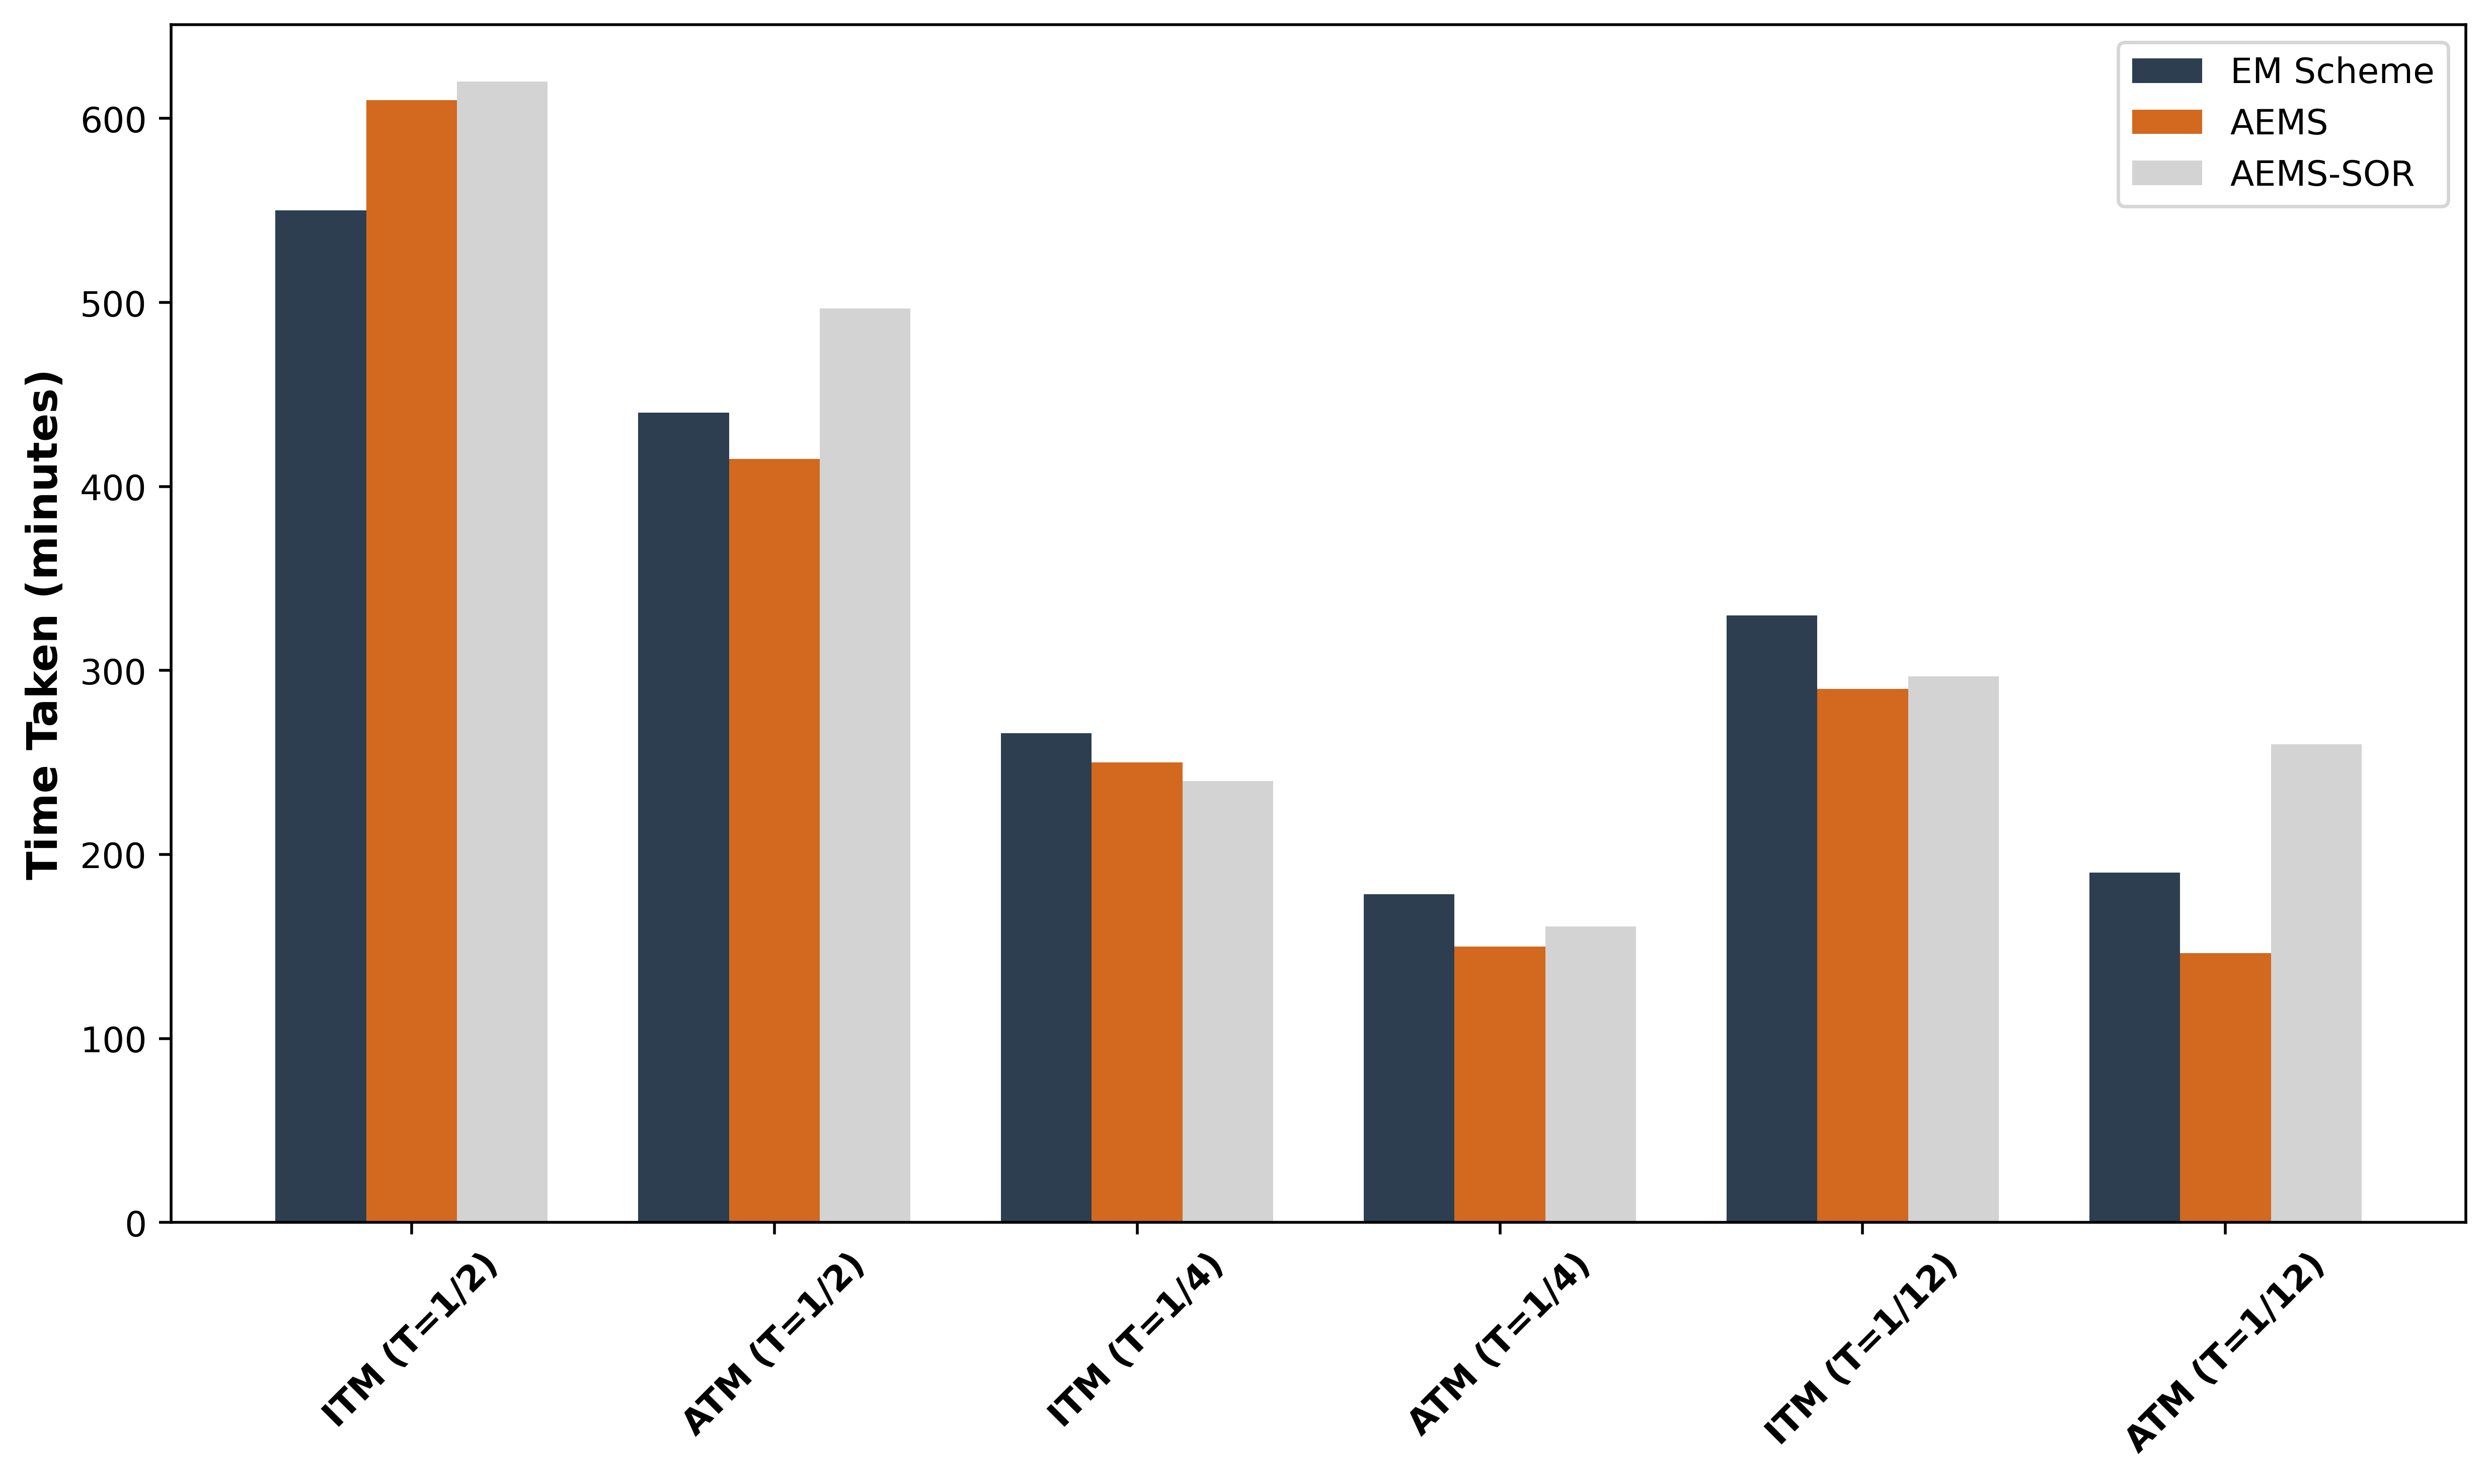
\includegraphics[width=0.75\textwidth]{../images/CompTime.png}
\caption{Total computation times over 10 independent simulation runs for selected American vanilla puts.}
\label{fig:comptime-vanilla}
\end{figure}



To illustrate the error behavior, Figures~\ref{fig:ITMvanilla}--\ref{fig:OTMvanilla} show relative errors for ITM, ATM, and OTM cases, respectively, plotted against the number of time steps. In most experiments, AEMS-SOR achieves lower errors than the EM scheme, particularly when $T = 1/4$ or $T=1/2$. AEMS also provides an improvement over EM, especially in the ATM case, where the option price is more sensitive to variance dynamics. However, for OTM options, when $T = 1/4$, EM shows lower errors than AEMS and AEMS-SOR, suggesting that higher-order schemes do not always provide improvements in this setting.

For OTM options ($K=90$), where the put option has a relatively low intrinsic value far from the strike, the numerical benefit of higher-order schemes is less pronounced. While both AEMS and AEMS-SOR outperform EM in terms of relative errors for larger $T$, for $T = 1/4$, EM achieves lower errors than AEMS and AEMS-SOR. Consequently, the improvements from AEMS-based schemes are more modest compared to ATM and ITM cases.  

ATM options ($K=100$) show the greatest sensitivity to numerical approximation. In this scenario, AEMS and AEMS-SOR generally reduce the error relative to EM, but for small time steps at $T = 1/12$, EM achieves comparable or slightly lower errors. AEMS-SOR remains the most accurate scheme overall, especially for larger $T$, where it consistently outperforms EM and AEMS.  

For ITM options ($K=110$), where the payoff is more stable and less path-dependent near expiry, all three schemes show similar convergence behavior as the number of time steps increases. AEMS-SOR achieves the lowest errors, though the differences between methods are relatively small for large time steps. This demonstrates its effectiveness even in less sensitive conditions, although the advantage over EM is less significant than in the ATM case.  




\begin{figure}[H]
\centering

\includegraphics[width=0.95\textwidth]{../images/ITM vanilla.png}
\caption{Relative error for ITM American vanilla put options as a function of time steps.}
\label{fig:ITMvanilla}
\end{figure}

\begin{figure}[H]
\centering

\includegraphics[width=0.95\textwidth]{../images/ATM vanilla.png}
\caption{Relative error for ATM American vanilla put options as a function of time steps.}
\end{figure}

\begin{figure}[H]
\centering

\includegraphics[width=0.95\textwidth]{../images/OTM vanilla.png}
\caption{Relative error for OTM American vanilla put options as a function of time steps.}
\label{fig:OTMvanilla}
\end{figure}


The AEMS-SOR scheme demonstrates robust convergence behavior, achieving the lowest relative errors for American vanilla put options across various maturities and moneyness conditions. AEMS also consistently improves upon the standard EM scheme, providing a favorable balance between accuracy and computational efficiency. While the advantages of AEMS and AEMS-SOR are most pronounced for ATM and ITM options, their benefits are less significant for OTM options, particularly when $T = 1/4$, where EM exhibits lower errors. For larger time steps (beyond approximately 70–100), AEMS-SOR stabilizes and approaches near-asymptotic performance.








\subsection{American Barrier Down-and-Out Put Option}

This barrier option becomes worthless (i.e., "knocked out") if the underlying asset's price falls below a predetermined level, referred to as the "barrier level," at any time during the life of the option.

For a down-and-out put option, the payoff at time $t\in [0,T]$, given that the option has not been knocked out, is:
\begin{equation*}
    \begin{cases}
        \max \left(K-S_t, 0\right) & \text { if } S_\tau \geq B \  \forall \tau \in[0, t] \\
        0 & \text { otherwise. }
    \end{cases}
\end{equation*}
For the parameters, in addition to preserving the same parameters in Table~\ref{tab:modelparameters}, we use a barrier value of $B = 90$.

Note that in this example of a down-and-out put option, we only consider two moneyness types (ATM and ITM) since the OTM option value is always zero; the barrier level $B=90$ causes the option to be knocked out immediately at $t=0$.



Tables~\ref{tab:OneMonthBarrier}--\ref{tab:ThreeMonthsBarrier} present the simulated option prices for different maturities and time steps using the AEMS, AEMS-SOR, and EM schemes. Values in parentheses indicate the percentage relative error compared to the benchmark.





\begin{table}[H]
    \centering
    \caption{American Barrier Down-and-Out Put Option Simulation Values ($T=1/12$)}
    \label{tab:OneMonthBarrier}
    \setlength{\tabcolsep}{4.6pt} 
    \begin{tabular}{cccccc}
        \toprule
        \textbf{Time Steps} & \textbf{Moneyness} & \textbf{AEMS} & \textbf{AEMS-SOR} & \textbf{EM} & \textbf{Benchmark} \\
        \midrule
        12 & ATM & 1.9246 (29.40) & 1.9989 (34.39) & 1.9601 (31.57) &  \\
        50 & ATM & 1.6132 (8.46) & 1.6955 (13.99) & 1.6892 (13.57) \\
        70 & ATM & 1.5414 (3.63) & 1.6265 (9.35) & 1.6289 (9.52) \\
        100 & ATM & 1.4723 (0.67) & 1.5556 (4.59) & 1.5584 (4.78) & 1.4873 \\
        \midrule
        12 & ITM & 8.3223 (7.72) & 8.4069 (8.79) & 8.3684 (8.30) &  \\
        50 & ITM & 7.8716 (1.87) & 7.9591 (3.00) & 7.9477 (2.85) \\
        70 & ITM & 7.8071 (1.03) & 7.8903 (2.11) & 7.8888 (2.09) \\
        100 & ITM & 7.7029 (0.03) & 7.7980 (0.91) & 7.8043 (1.00) & 7.7270 \\
        \bottomrule
    \end{tabular}
\end{table}

\begin{table}[H]
    \centering
    \caption{American Barrier Down-and-Out Put Option Simulation Values ($T=1/4$)}
    \setlength{\tabcolsep}{4.6pt} 
    \label{tab:ThreeMonthsBarrier}
    \begin{tabular}{cccccc}
        \toprule
        \textbf{Time Steps} & \textbf{Moneyness} & \textbf{AEMS} & \textbf{AEMS-SOR} & \textbf{EM} & \textbf{Benchmark} \\
        \midrule
        12 & ATM & 1.4548 (32.61) & 1.5096 (37.61) & 1.4589 (32.98) &  \\
        50 & ATM & 1.2391 (12.95) & 1.2610 (14.94) & 1.2668 (15.47) \\
        70 & ATM & 1.1669 (6.37) & 1.1972 (9.13) & 1.2064 (9.97) \\
        100 & ATM & 1.1121 (1.37) & 1.1383 (3.76) & 1.1473 (4.58) & 1.0970 \\
        \midrule
        12 & ITM & 5.8172 (3.28) & 5.9935 (6.41) & 5.9405 (5.47) &  \\
        50 & ITM & 5.7849 (2.70) & 5.8992 (4.73) & 5.9174 (5.06) \\
        70 & ITM & 5.7097 (1.37) & 5.8337 (3.57) & 5.8670 (4.16) \\
        100 & ITM & 5.6482 (0.28) & 5.7834 (2.68) & 5.8014 (3.00) & 5.6323 \\
        \bottomrule
    \end{tabular}
\end{table}

Figures~\ref{fig:BarrierITM} and~\ref{fig:BarrierATM} illustrate the relative error in percentage for ITM and ATM American barrier down-and-out put options. The performance of AEMS-SOR varies depending on the maturity and number of time steps. 

For ITM options (Figure~\ref{fig:BarrierITM}), AEMS-SOR achieves lower relative errors than EM across all maturities. However, for short maturities ($T = 1/12$), AEMS consistently produces the smallest errors. As the maturity increases, AEMS-SOR gradually outperforms EM, with noticeable improvements for $T = 1/4$ and $T = 1/2$. Notably, AEMS-SOR stabilizes more effectively for larger time steps.


\begin{figure}[H]
\centering

\includegraphics[width=0.95\textwidth,height=0.89\textheight,keepaspectratio]{../images/Barrier ITM.png}
\caption{Relative error for ITM American barrier down-and-out put options.}
\label{fig:BarrierITM}
\end{figure}

For ATM options (Figure~\ref{fig:BarrierATM}), AEMS performs the best for shorter maturities ($T = 1/12$), achieving the lowest errors among the three schemes. At $T = 1/4$, AEMS-SOR and AEMS demonstrate similar performance, both outperforming EM. For longer maturities ($T = 1/2$), AEMS-SOR initially shows higher errors but converges to a lower error rate than EM for larger time steps.


\begin{figure}[H]
\centering

\includegraphics[width=0.95\textwidth,height=0.89\textheight,keepaspectratio]{../images/Barrier ATM.png}
\caption{Relative error for ATM American barrier down-and-out put options.}
\label{fig:BarrierATM}
\end{figure}


Overall, AEMS-SOR provides significant improvements for medium to long maturities, particularly in ITM cases, where it stabilizes faster than EM. However, for shorter maturities, AEMS generally achieves the lowest errors, making it a competitive alternative. The refinement in AEMS-SOR is particularly effective at reducing numerical bias compared to EM in most cases.














\subsection{Forward Volatility Swap}\label{subsection:ForwardVolatilitySwap}

Forward volatility swaps under the Gatheral DMR model provide an effective means to capture future variance levels of the underlying asset. Following \cite{gatheral2008consistent}, the DMR model parameters (cf.\ Table~\ref{tab:modelparameters}) can be calibrated to markets such as VIX and SPX options. In \cite{bayer2013fast}, the authors further examined this calibration by analyzing variance swaps.

Under the DMR model, the $T$-maturity forward variance is
\begin{equation*}
   \xi_{t}(T) \;=\; \mathbb{E}[v_T \mid \mathcal{F}_t],
\end{equation*}
and the $T$-maturity variance swap is given by
\begin{equation*}
    \mathbb{E}\left.\left[\int_{t}^{T} v_{s}\,ds \, \right| \,  \mathcal{F}_t\right].
\end{equation*}
From \cite{bayer2013fast}, one obtains an explicit formula for the forward variance:
\begin{align*}
  \xi_{t}(T) &= \theta + (v_{t} - \theta)\, e^{-\kappa_1 \,\tau} + (v_{t}' - \theta)\,\frac{\kappa_1}{\kappa_1 - \kappa_2} 
  \bigl(e^{-\kappa_2\,\tau} - e^{-\kappa_1\,\tau}\bigr).
\end{align*}
where $\tau = T - t$. Integrating $\xi_t(T)$ over $[t, T]$ yields the analytical benchmark for the variance swap:
\begin{align*}
    \mathbb{E}\left.\left[\int_t^T v_{s}\,ds\, \right| \, \mathcal{F}_t\right]
    &= \theta\,\tau 
    + (v_t - \theta)\,\frac{1 - e^{-\kappa_1\,\tau}}{\kappa_1} \\
    &\quad + (v_t' - \theta)\,\frac{\kappa_1}{\kappa_1 - \kappa_2}
    \left\{
      \frac{1 - e^{-\kappa_2\,\tau}}{\kappa_2}
      - \frac{1 - e^{-\kappa_1\,\tau}}{\kappa_1}
    \right\}.
\end{align*}


In this subsection, we evaluate the performance of the AEMS, AEMS-SOR, and the EM scheme in pricing forward volatility swaps over longer maturities, namely $T=1$, $T=3$, and $T=10$ years. We simulate from $t=0$ using the same model parameters shown in Table~\ref{tab:modelparameters}, varying the time step sizes for each maturity. The analytical expression above serves as our benchmark.

Table~\ref{tab:volswap} presents the simulation results, with the numbers in parentheses indicating the percentage relative errors (\%) compared to the benchmark. Figure~\ref{fig:forwardswap} illustrates the convergence behavior in terms of relative error for each scheme as the number of time steps increases.

\begin{table}[H]
    \centering
    \caption{Forward volatility swap simulation values. Numbers in parentheses are relative errors (\%) from the benchmark.}
    \label{tab:volswap}
    \setlength{\tabcolsep}{4.6pt} 
    \begin{tabular}{c c c c c c}
        \toprule
        \textbf{Maturity} & \textbf{Time Steps} & \textbf{AEMS} & \textbf{AEMS-SOR} & \textbf{EM}&\textbf{Benchmark} \\
        \midrule
        $T=1$ & 50  & 0.0355 (1.81) & 0.0359 (2.89) & 0.0358 (2.75) \\
         & 100 & 0.0352 (1.01) & 0.0354 (1.46) & 0.0354 (1.39) \\
        & 200 & 0.0351 (0.56) & 0.0351 (0.71) & 0.0351 (0.77) \\
         & 300 & 0.0349 (0.07) & 0.0350 (0.52) & 0.0351 (0.59)&0.0348 \\
        \midrule
        $T=3$ & 50  & 0.1128 (2.24) & 0.1182 (7.12) & 0.1183 (7.21) \\
        & 100 & 0.1118 (1.27) & 0.1147 (3.96) & 0.1148 (4.02) \\
        & 200 & 0.1110 (0.61) & 0.1129 (2.28) & 0.1129 (2.30) \\
        & 300 & 0.1109 (0.47) & 0.1124 (1.80) & 0.1124 (1.77) &0.1103\\
        \midrule
        $T=10$ & 100 & 0.3973  (1.88) & 0.4291 (12.78) & 0.4295 (10.73) \\
        & 200 & 0.3940  (1.02) & 0.4122 (5.70)  & 0.4124 (5.75)  \\
        & 300 & 0.3932  (0.81) & 0.4066 (4.26)  & 0.4063 (4.19)  \\
         & 500 & 0.3909  (0.23) & 0.4002 (2.62)  & 0.3989 (2.29) &0.3900 \\
        \bottomrule
    \end{tabular}
\end{table}


\begin{figure}[H]
\centering

\includegraphics[width=0.85\textwidth,keepaspectratio]{../images/Forward swap.png}
\caption{Relative error for forward volatility swap.}
\label{fig:forwardswap}
\end{figure}

Across all maturities and time steps, the AEMS scheme consistently exhibits the lowest relative errors, highlighting its robust performance in approximating the forward variance integral. Specifically, for $T=1$ and $T=3$, AEMS converges more rapidly to the benchmark solution than the other two methods, often achieving relative errors below $0.5\%$ when sufficiently many time steps are used. 

By contrast, AEMS-SOR, despite its second-order refinement, shows similar error levels to the EM scheme for larger maturities, especially at $T=10$. Although the refined scheme uses higher-order corrections, the cumulative effect of variance integration over long horizons appears to diminish the benefit of these local adjustments. As a result, AEMS-SOR does not consistently outperform EM in scenarios with extensive time-to-maturity.

All three schemes demonstrate decreasing errors as the number of time steps increases, confirming convergence. However, AEMS provides the most significant reduction, underscoring its advantage in precision for forward volatility swap pricing. These observations align with the intuitive notion that an adaptive approach to simulating the variance process, as found in AEMS, can more effectively capture the time-dependent features of the DMR model, yielding higher accuracy than standard first-order EM or AEMS-SOR fixed-step refinements.

Overall, these results confirm the effectiveness of AEMS in achieving superior accuracy for forward volatility swaps, particularly for moderate and shorter maturities, and validate its applicability as a reliable numerical scheme under the Gatheral DMR model.





\subsection{Basket Option of Two Assets}

A basket option is a financial derivative whose payoff depends on the performance of a group (or "basket") of underlying assets. These options are particularly useful for investors who wish to hedge or speculate on a portfolio of assets collectively rather than individually.

For a basket option involving two stocks, the payoff depends on the combined performance of these stocks, weighted by predefined factors. There are two standard approaches for computing the payoff:
\begin{itemize}
    \item \textbf{Weighted Sum Method:} In this approach, each stock in the basket has a weight that reflects its contribution to the basket’s total value. The payoff formula for a put option using the weighted sum is given by:
    \begin{equation*}
    \text{Payoff} = \max\left[K - (a_1 S_1(T) + a_2 S_2(T)), 0\right],        
    \end{equation*}
    where $a_1$ and $a_2$ are the weights of stock 1 ($S_1$) and stock 2 ($S_2$), respectively, and $K$ is the strike price of the option.
    
    \item \textbf{Weighted Average Method:} This method is used when the weights represent the proportion of the total investment in each asset. The payoff is based on the average price of the stocks in the basket, given by:
    \begin{equation*}
    \text{Payoff} = \max\left[K - \frac{a_1 S_1(T) + a_2 S_2(T)}{a_1 + a_2}, 0\right].
    \end{equation*}
    In this example, we assume equal weighting for both assets, setting $a_1 = a_2 = \frac{1}{2}$. Under this assumption, the weighted average and the weighted sum formulations yield the same results.
\end{itemize}

We conduct numerical experiments with initial stock prices $S_{1}(0) = S_{2}(0) = 100$, a strike price $K = 110$, a risk-free rate $r = 0.05$, and a maturity of $T = 1/4$. While the model parameters for the first asset remain unchanged from previous experiments, we modify the model parameters for the second asset $S_2$ as specified in Table~\ref{tab:parameters}.


\begin{table}[H]
\centering
\setlength{\tabcolsep}{6pt} % Adjusts column spacing
\caption{DMR model parameters for the second asset $S_2$.}
\label{tab:parameters}
\begin{tabular*}{\textwidth}{@{\extracolsep{\fill}} ccccc ccccc}
\toprule
$v^{S_2}_{0}$ & $v^{\prime^{S_2}}_{0}$ & $\kappa^{S_2}_{1}$ & $\kappa^{S_2}_{2}$ & $\theta^{S_2}$ & $\xi^{S_2}_{1}$ & $\xi^{S_2}_{2}$ & $\rho^{S_2}_{12}$ & $\rho^{S_2}_{13}$ & $\rho^{S_2}_{23}$ \\
\midrule
$0.114$ & $0.09$ & 1 & 0.5 & 0.09 & 1 & 0.502 & $-0.3$ & $-0.727$ & 0.59 \\ 
\bottomrule
\end{tabular*}
\end{table}


Figure~\ref{fig:basket} compares the consistency of option pricing across multiple runs using the EM, AEMS, and AEMS-SOR. The simulation consists of 50 time steps per run across 30 independent trials.

\begin{figure}[H]
    \centering
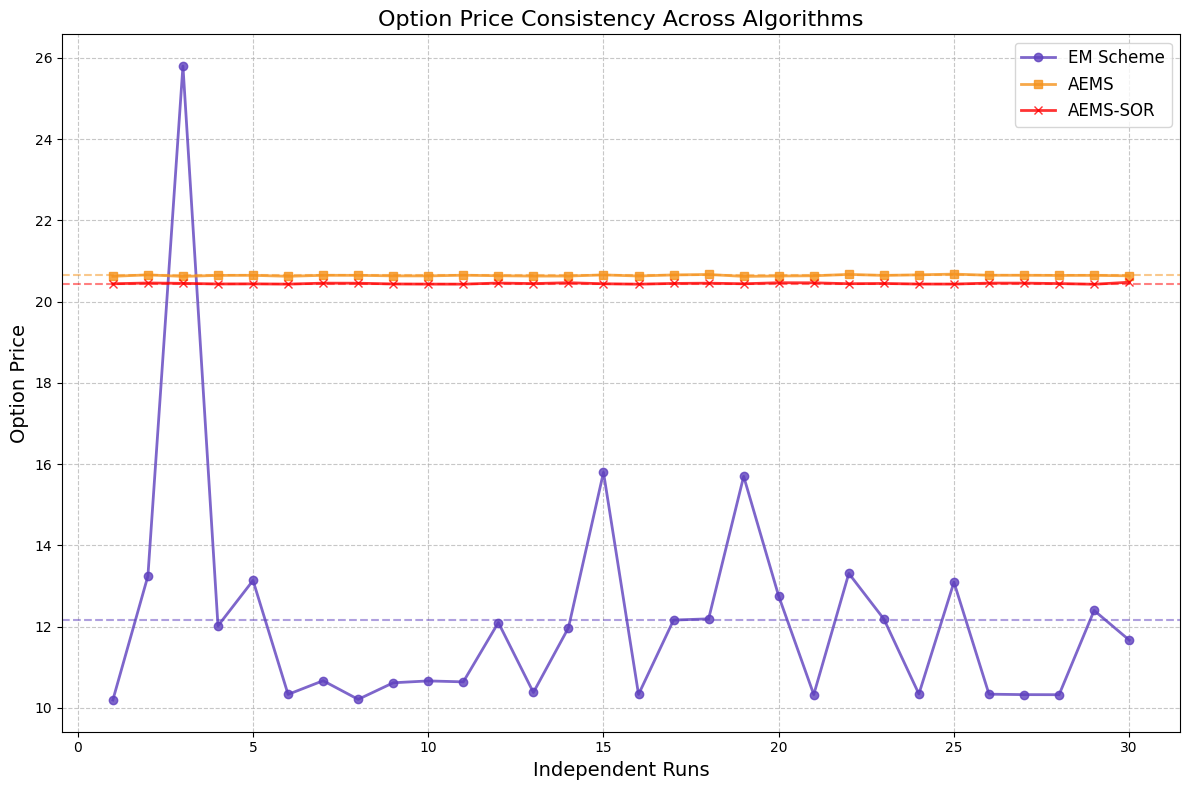
\includegraphics[width=0.95\textwidth,height=0.95\textheight,keepaspectratio]{../images/basket option.png}
    \caption{Comparison of pricing stability for basket options using EM, AEMS, and AEMS-SOR.}
    \label{fig:basket}
\end{figure}

The results highlight the inconsistency of the EM scheme, which shows significant fluctuations across independent runs. In contrast, AEMS and AEMS-SOR provide superior stability, producing consistent and reliable option prices with minimal deviations. The sharp fluctuations in the EM scheme emphasize its limitations in multi-asset pricing applications.

AEMS and AEMS-SOR enhance both accuracy and stability, making them more suitable for financial applications that require precision and consistency. The second-order refinement in AEMS-SOR further strengthens its robustness, ensuring more reliable valuations for basket options.






\section{Conclusion}

This paper analyzes the Almost-Exact Mixed (Simulation) Scheme (AEMS) and its second-order refinement (AEMS-SOR) as efficient numerical methods for simulating the Gatheral DMR model and pricing derivatives. The Gatheral DMR model extends traditional stochastic volatility frameworks by incorporating a secondary mean-reverting variance process, necessitating robust numerical schemes due to its non-affine structure.

AEMS improves variance path simulation accuracy using the AES methodology with a Milstein correction, while AEMS-SOR enhances weak convergence properties through second-order refinements. Our results show that both schemes outperform the Euler-Maruyama (EM) method in accuracy and stability across a range of derivatives.

Numerical experiments demonstrate that AEMS and AEMS-SOR achieve faster convergence and lower errors for American vanilla and barrier put options, particularly for at-the-money and in-the-money contracts with longer maturities. However, for short-maturity out-of-the-money options, EM may exhibit smaller errors. For forward volatility swaps, AEMS provides consistently lower relative errors, though AEMS-SOR’s benefits are less pronounced for long maturities. In two-asset basket options, both AEMS and AEMS-SOR yield more stable pricing results compared to EM.

Overall, AEMS achieves significant accuracy improvements with minimal computational overhead, while AEMS-SOR further enhances numerical stability where higher precision is required. These findings establish AEMS and AEMS-SOR as efficient approaches for pricing derivatives under the Gatheral DMR model.







\section*{Appendix}
%\addcontentsline{toc}{section}{Appendix}

\begin{algorithm}[H]
\caption{AEMS Scheme for Gatheral DMR Model}
\label{alg:AEMS}
\begin{algorithmic}[1]
\State \textbf{Input:} $N$: Number of paths, $M$: Number of steps, $T$: Time to maturity, $r$, $S_0$, $\kappa_1$, $\kappa_2$, $\xi_1$, $\xi_2$, $\rho_{12}$, $\rho_{13}$, $\rho_{23}$, $\theta$, $v_0$, $v_0'$: Model parameters.
\State Initialize $v = v_0$, $v^{'} = v_0'$, $X_{0} = \ln(S_0)$, $\Delta t = \frac{T}{M}$
\For{$i = 0$ to $M-1$}
    \State Generate Wiener processes $W^{(1)}, W^{(2)}, W^{(3)}$. 
    \State Compute $v^{'}_{i+1}$ using CIR Sampling:
    \[
    \delta = \frac{4 \kappa_2 \theta}{\xi_2^2}, \quad c = \frac{\xi_2^2 (1 - e^{-\kappa_2 \Delta t})}{4 \kappa_2}, \quad
    \bar{\kappa} = \frac{4 \kappa_2 v^{'}_{i} e^{-\kappa_2 \Delta t}}{\xi_2^2 (1 - e^{-\kappa_2 \Delta t})}.
    \]
    \[
    v^{'}_{i+1} = c \cdot \chi^2_{\delta}(\bar{\kappa})
    \]
    \State Update $v^{'}_{i+1}$ using truncation
    \[
    v^{'}_{i+1} = \max\left(v^{'}_{i+1},0\right)
    \]
    \State Update $v_{i+1}$:
    \[
    v_{i+1} = v_{i} + \kappa_1 \left(v^{'}_{i} - v_{i}\right) \Delta t + \xi_1 \sqrt{v_{i}} \left(W^{(2)}_{i+1} - W^{(2)}_{i}\right) + \frac{1}{4} \xi_1^2 \left(\left(W^{(2)}_{i+1} - W^{(2)}_{i}\right)^2 - \Delta t\right)
    \]
    \State Compute $\rho^{*}$ and $\rho^{**}$
    \[
    \rho^*=\sqrt{\left(1-\rho^2_{13}-\frac{(\rho_{12}-\rho_{13}\rho_{23})^2}{1-\rho^2_{23}}\right)},\quad \rho^{**}=\left(\frac{\rho_{12}-\rho_{13}\rho_{23}}{\sqrt{1-\rho^2_{23}}}\,-\rho_{13}\frac{\sqrt{1-\rho_{23}^2}}{\rho_{23}}\right)
    \]
    \State Update $X^{i+1}$:
    \[
    \begin{aligned}
        X_{i+1} = X_{i} + \left(r-\frac{1}{2}v_{i}\right)\Delta t + &\rho^*  \sqrt{v_{i}}\left(W^{(2)}_{i+1}-W^{(2)}_{i}\right)+\rho^{**} \sqrt{v_{i}}\left(W^{(2)}_{i+1}-W^{(2)}_{i}\right)\\
        +&\rho_{13}\left(\frac{v_{i+1}-v_{i}-\kappa_1(v_{i}^{'}-v_{i})\Delta t}{\xi_1 \rho_{23}}\right)
    \end{aligned}
    \]
\EndFor
\State Compute $S = e^X$
\State \textbf{Return:} $S, v, v^{'}$
\end{algorithmic}
\end{algorithm}

\begin{algorithm}[H]
\caption{AEMS-SOR Scheme for Gatheral DMR Model}
\label{alg:AEMS-SOR}
\begin{algorithmic}[1]
\State \textbf{Input:} $N$: Number of paths, $M$: Number of steps, $T$: Time to maturity, $r$, $S_0$, $\kappa_1$, $\kappa_2$, $\xi_1$, $\xi_2$, $\rho_{12}$, $\rho_{13}$, $\rho_{23}$, $\theta$, $v_0$, $v_0'$: Model parameters.
\State Initialize $v = v_0$, $v^{'} = v_0'$, $X_{0} = \ln(S_0)$, $\Delta t = \frac{T}{M}$
\For{$i = 0$ to $M-1$}
    \State Generate Wiener processes $W^{(1)}, W^{(2)}, W^{(3)}$.
    \State Update the variance process $v^{'}$:
    \[
    v^{'}_{i+1} = v^{'}_{i} + \kappa_2 (\theta - v^{'}_{i}) \Delta t + \xi_2 \sqrt{v^{'}_{i}} (W^{(3)}_{i+1} - W^{(3)}_{i})
    \]
    \State Apply truncation to ensure non-negativity:
    \[
    v^{'}_{i+1} = \max(0, v^{'}_{i+1})
    \]
    \State Update $v_{i+1}$:
    \[
    v_{i+1} = v_{i} + \kappa_1 (v^{'}_{i} - v_{i}) \Delta t + \xi_1 \sqrt{v_{i}} (W^{(2)}_{i+1} - W^{(2)}_{i})
    \]
    \State Apply truncation to ensure non-negativity:
    \[
    v_{i+1} = \max(0, v_{i+1})
    \]
    \State Update the logarithm of the asset price $X$:
    \[
    X_{i+1} = X_i + \left(r - \frac{1}{2} v_{i}\right) \Delta t + \sqrt{v_{i}} (W^{(1)}_{i+1} - W^{(1)}_{i})
    \]
    \State Add higher order corrections to the simulated $X$:
    \[
    X_{i+1} += \left(\left(r - \frac{1}{2} v_i\right) \frac{1}{2} \sqrt{v_i} - \frac{1}{8} \sqrt{v_i}\right) (W^{(1)}_{i+1} - W^{(1)}_{i}) \Delta t - (\Delta t (W^{(1)}_{i+1} - W^{(1)}_{i}) / 2)
    \]
    \[
    X_{i+1} += (r - \frac{1}{2}) \sqrt{v_i} (\Delta t (W^{(1)}_{i+1} - W^{(1)}_{i}) / 2) + \frac{1}{4} ((W^{(1)}_{i+1} - W^{(1)}_{i})^2 - \Delta t)
    \]
    \[
    X_{i+1} += (r^2 - \frac{1}{2} r - \frac{1}{2} v_i r + \frac{1}{4} v_i) \frac{1}{2} \Delta t^2
    \]
    \State Ensure non-negativity for $X$:
    \[
    X_{i+1} = \max(0, X_{i+1})
    \]
\EndFor
\State Compute the asset price $S$ from the logarithm of $X$:
\[
S = e^X
\]
\State \textbf{Return:} $S, v, v^{'}$
\end{algorithmic}
\end{algorithm}




%%%%%%%%%%%%%%%%%%%%%%%% referenc.tex %%%%%%%%%%%%%%%%%%%%%%%%%%%%%%
% sample references
% %
% Use this file as a template for your own input.
%
%%%%%%%%%%%%%%%%%%%%%%%% Springer-Verlag %%%%%%%%%%%%%%%%%%%%%%%%%%
%
% BibTeX users please use
% \bibliographystyle{}
% \bibliography{}
%
%\biblstarthook{

\begin{thebibliography}{99.}%
% Contribution
\bibitem{albuhayri2021asymptotics} Albuhayri, M., Malyarenko, A., Silvestrov, S., Ni, Y., Engström, C., Tewolde, F., Zhang, J.: Asymptotics of implied volatility in the Gatheral double stochastic volatility model. Appl. Model. Tech. Data Anal. \textbf{8}, 27--38 (2021). Wiley Online Library

% Journal article
\bibitem{bayer2013fast} Bayer, C., Gatheral, J., Karlsmark, M.: Fast Ninomiya--Victoir calibration of the double-mean-reverting model. Quant. Finance. \textbf{13}(11), 1813--1829 (2013). Taylor \& Francis
% Journal article
\bibitem{black1973pricing} Black, F., Scholes, M.: The pricing of options and corporate liabilities. J. Polit. Econ. \textbf{81}(3), 637--654 (1973). The University of Chicago Press.


% Contribution
\bibitem{gatheral2008consistent} Gatheral, J.: Consistent modeling of SPX and VIX options. In: Bachelier Congress, vol. 37, pp. 39--51 (2008)

% Monograph
\bibitem{gatheral2011volatility} Gatheral, J.: The volatility surface: A practitioner's guide. John Wiley \& Sons, New York (2011)



% Journal article
\bibitem{kalicanin2022bermudan}
 Kalicanin Dimitrov, M., Dimitrov, M., Malyarenko, A., Ni, Y.: Almost-exact simulation scheme for Heston-type models: Bermudan and American option pricing. [Manuscript submitted for publication] (2025).



% Monograph
\bibitem{oosterlee2019mathematical} Oosterlee, C.W., Grzelak, L.A.: Mathematical modeling and computation in finance: With exercises and Python and MATLAB computer codes. World Scientific, Singapore (2019)

% Journal article
\bibitem{kil2022closed} Kil, H.-M., Kim, J.-H.: A closed-form approximation formula for pricing European options under a three-factor model. Prob. Eng. Inform. Sci. \textbf{36}(4), 1214--1240 (2022). Cambridge University Press

% Journal article
\bibitem{cox1976valuation} Cox, J.C., Ross, S.A.: The valuation of options for alternative stochastic processes. J. Financial Econ. \textbf{3}(1-2), 145--166 (1976). Elsevier

% Journal article
\bibitem{heston1993closed} Heston, S.L.: A closed-form solution for options with stochastic volatility with applications to bond and currency options. Rev. Financial Stud. \textbf{6}(2), 327--343 (1993). Oxford University Press

% Journal article
\bibitem{hagan2002managing} Hagan, P.S., Kumar, D., Lesniewski, A.S., Woodward, D.E.: Managing smile risk. Best of Wilmott. \textbf{1}, 249--296 (2002)

% Journal article
\bibitem{mil1975approximate} Milstein, G.N.: Approximate integration of stochastic differential equations. Theory Probab. Appl. \textbf{19}(3), 557--562 (1975). SIAM

% Journal article
\bibitem{christoffersen2009shape} Christoffersen, P., Heston, S., Jacobs, K.: The shape and term structure of the index option smirk: Why multifactor stochastic volatility models work so well. Manag. Sci. \textbf{55}(12), 1914--1932 (2009). INFORMS

% Journal article
\bibitem{fadugba2013convergence} Fadugba, S.E., Adegboyegun, B.J., Ogunbiyi, O.T.: On the convergence of Euler--Maruyama method and Milstein scheme for the solution of stochastic differential equations. Int. J. Appl. Math. Model. \textbf{1}(0), 1 (2013)

% Online Document
\bibitem{giles2013analysis} Giles, M.B., Debrabant, K., Rößler, A.: Analysis of multilevel Monte Carlo path simulation using the Milstein discretisation. arXiv preprint arXiv:1302.4676 (2013)

% Monograph
\bibitem{hilpisch2015derivatives} Hilpisch, Y.: Derivatives Analytics with Python. John Wiley \& Sons, New York (2015)

% Monograph
\bibitem{glasserman2004monte} Glasserman, P.: Monte Carlo methods in financial engineering. Springer, Berlin (2004)

% Journal article
\bibitem{van2010efficient} Van Haastrecht, A., Pelsser, A.: Efficient, almost exact simulation of the Heston stochastic volatility model. Int. J. Theor. Appl. Finance. \textbf{13}(01), 1--43 (2010). World Scientific

% Monograph
\bibitem{hull2003options} Hull, J.C.: Options futures and other derivatives. Pearson Education, India (2003)

% Monograph
\bibitem{kwok2008mathematical} Kwok, Y.-K.: Mathematical models of financial derivatives. Springer, Berlin (2008)

% Journal article
\bibitem{longstaff2001valuing} Longstaff, F.A., Schwartz, E.S.: Valuing American options by simulation: A simple least-squares approach. Rev. Financial Stud. \textbf{14}(1), 113--147 (2001). Oxford University Press

% Journal article
\bibitem{huh2018scaled} Huh, J., Jeon, J., Kim, J.: A scaled version of the double-mean-reverting model for VIX derivatives. Math. Financial Econ. \textbf{12}, 495--515 (2018). Springer

% Monograph
\bibitem{roman2017analytical} Röman, J.R.M.: Analytical finance. Springer, Berlin (2017)

% Monograph
\bibitem{golub2013matrix} Golub, G.H., Van Loan, C.F.: Matrix computations. JHU Press, Baltimore (2013)

% Journal article
\bibitem{benchmark_test1} Zhang, S.M., Feng, Y.: American option pricing under the double Heston model based on asymptotic expansion. Quant. Finance. \textbf{19}(2), 211--226 (2019). Taylor \& Francis

% Journal article
\bibitem{benchmark_test2} Medvedev, A., Scaillet, O.: Pricing American options under stochastic volatility and stochastic interest rates. J. Financial Econ. \textbf{98}(1), 145--159 (2010). Elsevier

% Journal article
\bibitem{mil1979method} Milstein, G.N.: A method of second-order accuracy integration of stochastic differential equations. Theory Probab. Appl. \textbf{23}(2), 396--401 (1979). SIAM

% Contribution
\bibitem{talay1984efficient} Talay, D.: Efficient numerical schemes for the approximation of expectations of functionals of the solution of an SDE, and applications. In: Filtering and Control of Random Processes, pp. 294--313. Springer, Paris (1984)

% Journal article
\bibitem{broadie2006exact} Broadie, M., Kaya, Ö.: Exact simulation of stochastic volatility and other affine jump diffusion processes. Oper. Res. \textbf{54}(2), 217--231 (2006). INFORMS

% Monograph
\bibitem{hirsa2013computational} Hirsa, A.: Computational methods in finance. CRC Press, Boca Raton (2013)
\end{thebibliography}

\end{document}
